% 这是中国科学院大学计算机科学与技术专业《计算机组成原理(研讨课)》使用的实验报告 Latex 模板
% 本模板与 2024 年 2 月 Jun-xiong Ji 完成, 更改自由 Shing-Ho Lin 和 Jun-Xiong Ji 于 2022 年 9 月共同完成的基础物理实验模板
% 如有任何问题, 请联系: jijunxoing21@mails.ucas.ac.cn
% This is the LaTeX template for report of Experiment of Computer Organization and Design courses, based on its provided Word template. 
% This template is completed on Febrary 2024, based on the joint collabration of Shing-Ho Lin and Junxiong Ji in September 2022. 
% Adding numerous pictures and equations leads to unsatisfying experience in Word. Therefore LaTeX is better. 
% Feel free to contact me via: jijunxoing21@mails.ucas.ac.cn

\documentclass[11pt]{article}

\usepackage[a4paper]{geometry}
\geometry{left=2.0cm,right=2.0cm,top=2.5cm,bottom=2.5cm}

\usepackage{ctex} % 支持中文的LaTeX宏包
\usepackage{amsmath,amsfonts,graphicx,subfigure,amssymb,bm,amsthm,mathrsfs,mathtools,breqn} % 数学公式和符号的宏包集合
\usepackage{algorithm,algorithmicx} % 算法和伪代码
\usepackage[noend]{algpseudocode} % 算法和伪代码
\usepackage{fancyhdr} % 自定义页眉页脚
\usepackage[framemethod=TikZ]{mdframed} % 创建带边框的框架
\usepackage{fontspec} % 字体设置
\usepackage{adjustbox} % 调整盒子大小
\usepackage{fontsize} % 设置字体大小
\usepackage{tikz,xcolor} % 绘制图形和使用颜色
\usepackage{multicol} % 多栏排版
\usepackage{multirow} % 表格中合并单元格
\usepackage{pdfpages} % 插入PDF文件
\usepackage{listings} % 在文档中插入源代码
\usepackage{wrapfig} % 文字绕排图片
\usepackage{bigstrut,multirow,rotating} % 支持在表格中使用特殊命令
\usepackage{booktabs} % 创建美观的表格
\usepackage{circuitikz} % 绘制电路图
\usepackage{zhnumber} % 中文序号(用于标题)
\usepackage{tabularx} % 表格折行

\definecolor{dkgreen}{rgb}{0,0.6,0}
\definecolor{gray}{rgb}{0.5,0.5,0.5}
\definecolor{mauve}{rgb}{0.58,0,0.82}
\lstset{
  frame=tb,
  aboveskip=3mm,
  belowskip=3mm,
  showstringspaces=false,
  columns=flexible,
  framerule=1pt,
  rulecolor=\color{gray!35},
  backgroundcolor=\color{gray!5},
  basicstyle={\small\ttfamily},
  numbers=none,
  numberstyle=\tiny\color{gray},
  keywordstyle=\color{blue},
  commentstyle=\color{dkgreen},
  stringstyle=\color{mauve},
  breaklines=true,
  breakatwhitespace=true,
  tabsize=3,
}

% 轻松引用, 可以用\cref{}指令直接引用, 自动加前缀. 
% 例: 图片label为fig:1
% \cref{fig:1} => Figure.1
% \ref{fig:1}  => 1
\usepackage[capitalize]{cleveref}
% \crefname{section}{Sec.}{Secs.}
\Crefname{section}{Section}{Sections}
\Crefname{table}{Table}{Tables}
\crefname{table}{Table.}{Tabs.}

% \setmainfont{Palatino Linotype.ttf}
% \setCJKmainfont{SimHei.ttf}
% \setCJKsansfont{Songti.ttf}
% \setCJKmonofont{SimSun.ttf}
\punctstyle{kaiming}
% 偏好的几个字体, 可以根据需要自行加入字体ttf文件并调用

\renewcommand{\emph}[1]{\begin{kaishu}#1\end{kaishu}}

% 对 section 等环境的序号使用中文
\renewcommand \thesection{\zhnum{section}、}
\renewcommand \thesubsection{\arabic{section}}


%%%%%%%%%%%%%%%%%%%%%%%%%%%
%改这里可以修改实验报告表头的信息
\newcommand{\name}{艾华春, 李霄宇, 王敬华}
\newcommand{\studentNum}{2022K8009916011,2022K8009929029,2022K8009925009}
\newcommand{\major}{计算机科学与技术}
\newcommand{\labNum}{7}
\newcommand{\labName}{高速缓存设计}
%%%%%%%%%%%%%%%%%%%%%%%%%%%

\begin{document}

\begin{center}
  \LARGE \bf 中国科学院大学 \\《计算机体系结构基础(研讨课)》实验报告
\end{center}

\begin{center}
  \emph{姓名} \underline{\makebox[10em][c]{\name}} \\
  % 如果名字比较长, 可以修改box的长度"8em"为其他值
  \emph{学号} \underline{\makebox[30em][c]{\studentNum}}\\
  % \emph{专业} \underline{\makebox[15em][c]{\major}}\\
  \emph{实验项目编号} \underline{\makebox[3em][c]{\labNum}}
  \emph{实验名称} \underline{\makebox[30em][c]{\labName}}\\
\end{center}

% \begin{center}
%   \begin{tabularx}{\textwidth}{|lX|}
%     \hline
%     注1: & 撰写此 Word 格式实验报告后以 PDF 格式保存 SERVE CloudIDE 的 \texttt{/home/serve-ide/ cod-lab/reports} 目录下(注意:reports 全部小写)。文件命名规则:\texttt{prjN.pdf},其中 \texttt{prj} 和后缀名 \texttt{pdf} 为小写,\texttt{N} 为1至4的阿拉伯数字。例如:\texttt{prj1.pdf}。PDF 文件大小应控制在 5MB 以内。此外,实验项目5包含多个选做内容,每个选做实验应提交各自的实验报告文件,文件命名规则:\texttt{prj5-projectname.pdf},其中``-''为英文标点符号的短横线。文件命名举例:\texttt{prj5-dma.pdf}。具体要求详见实验项目5讲义。 \\

%     注2: & 使用\texttt{git add}及\texttt{git commit}命令将实验报告\texttt{PDF}文件添加到本地仓库master分支,并通过\texttt{git push}推送到实验课SERVE GitLab远程仓库master分支(具体命令详见实验报告)。 \\

%     注3: & 实验报告模板下列条目仅供参考,可包含但不限定如下内容。实验报告中无需重复描述讲义中的实验流程。\\
%     \hline
%   \end{tabularx}
% \end{center}

  

\section{逻辑电路结构与仿真波形的截图及说明}
\noindent
$\bullet$
\textbf{Cache模块设计}。
\begin{enumerate}
    \item Cache 的逻辑组织结构
    
    Cache采用两路组相连的方式,每一路包含相同的tag,v表,d表,4个data\_bank表。所有的表同一时间只能接受
    一个读或写操作。
    
    如下图所示:
    \begin{figure}[H]
        \centering
        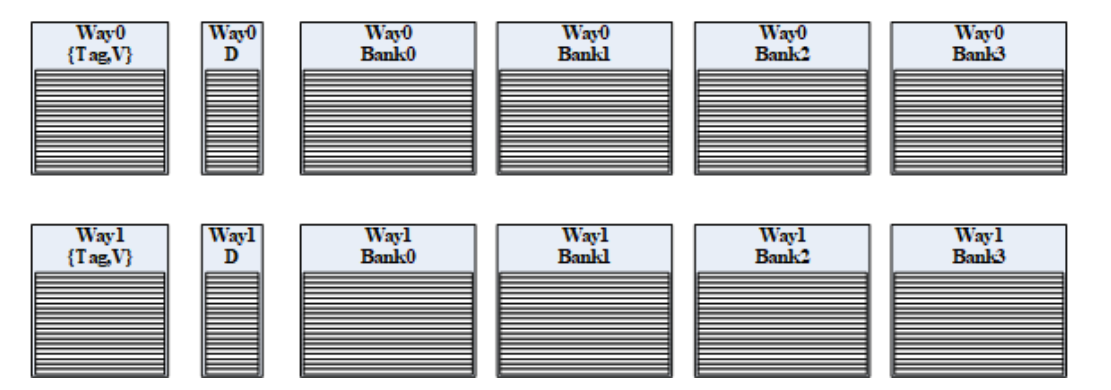
\includegraphics[width=0.8\textwidth]{fig/fig1.png}
        \caption{Cache逻辑组织结构}
        \label{fig:1}
    \end{figure}
    \begin{enumerate}
        \item data\_bank表
\begin{lstlisting}[language=verilog]
generate
for (i = 0; i < 4; i = i + 1)begin: data_way0
    data_bank_ram data_way0(
        .clka   (clk),
        .wea    (data_way0_wen[i]),   
        .addra  (data_way0_index[i]),
        .dina   (data_way0_wdata),
        .douta  (way0_data[i])  
    );
end
endgenerate
\end{lstlisting}
        一个Cache行有16个字节,分为4个data\_bank表。
        
        每一路的data\_bank表为一个RAM 256 * 32(深度*宽度)。

        \item tag,v表
\begin{lstlisting}[language=verilog]
    tagv_ram tagv_ram_way0 (
        .clka   (clk), 
        .wea    (tagv_way0_wen),
        .addra  (tagv_way0_index),
        .dina   ({tagv_way0_wdata}),
        .douta  ({way0_tag,way0_v})
    );
\end{lstlisting}    
        每个Cache行有一个tag和v域,表示该行是否有效和该行的在主存中的地址。

        由于所有Cache操作对tag和v的操作是完全一致的,所以,
        tag和v合并在一起存储,tag占高位,v占低位。
        
        每一路的tagv表用一个RAM 256 * 21(深度*宽度)存储。
        \item d表
    \begin{lstlisting}[language=verilog]
        d_regfile d_way0(
            .clk        (clk),
            .resetn     (resetn),
            .addr       (d_way0_index),
            .wen        (d_way0_wen),
            .wdata      (d_way0_wdata),
            .rdata      (way0_d)
        );   
    \end{lstlisting}
        每个Cache行有一个d域,表示该行的脏位,由于每行只有一个脏位,所以用regfile存储。

        每一路的d表用256个1位的寄存器堆存储。
    \end{enumerate}
    \item Cache的内部的控制逻辑设计
    \item 
    Cache 的控制包括两个状态机,主状态机和write buffer状态机。
    \begin{figure}[H]
        \centering
        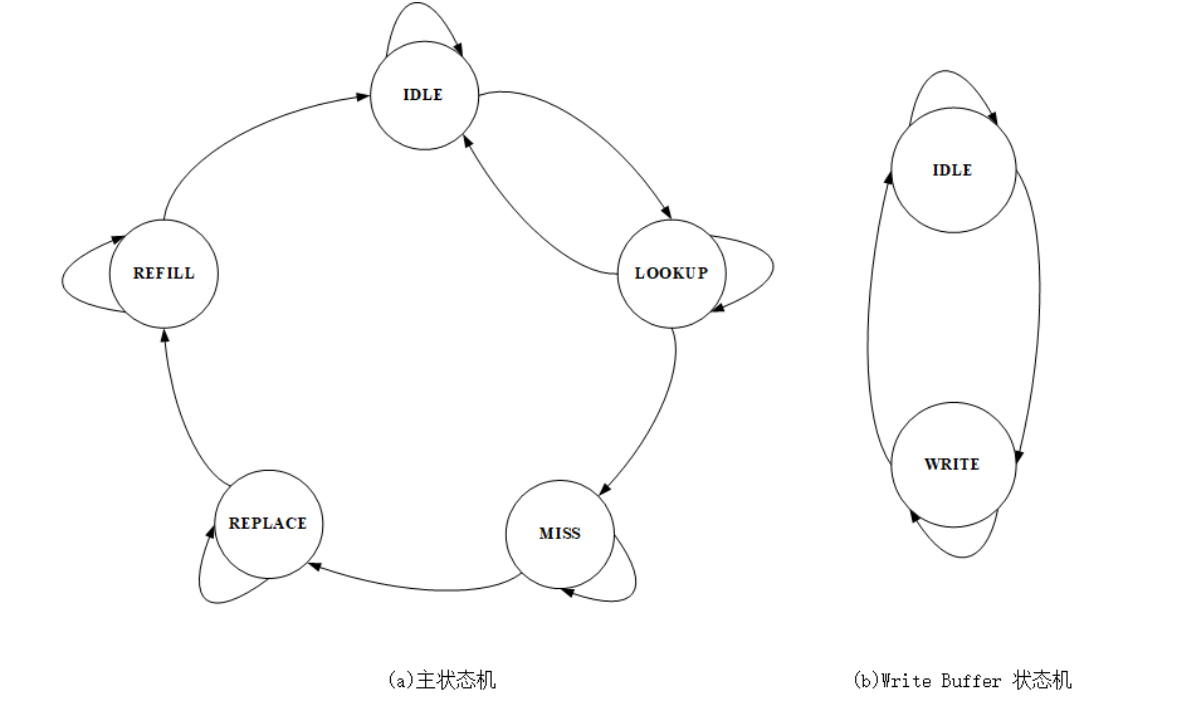
\includegraphics[width=0.8\textwidth]{fig/fig2.png}
        \caption{Cache的状态机}
        \label{fig:2}
    \end{figure}    
        
        主状态机包括5个状态,idle,lookup, miss, replace, refill。

        \begin{enumerate}
            \item idle状态
            
            在idle状态下,Cache等待外部的请求,当有请求到来,且与Cache中的Hit write不冲突时,用组合逻辑拉高addr\_ok信号,
            并在下一拍Cache进入lookup状态。
 \begin{lstlisting}[language=verilog]
assign addr_ok =    main_current_state == LOOKUP & cache_hit & ~hit_write_conflict
                    |main_current_state == IDLE & ~hit_write_conflict;
 \end{lstlisting}
 同时,将请求信息中的index通过组合逻辑,送到Cache进行查询,将两路的对应的Cache行的数据(tag, v, data)在下一拍读出来。

            并且,在request buffer中存储请求的相关信息。

\begin{lstlisting}[language=verilog]
// requeset buffer,存储接受到的请求信息
always @(posedge clk)begin
    if(~resetn) begin
        req_buffer_op <=       1'b0;
        req_buffer_index <=    8'b0;
        req_buffer_tag <=      20'b0;
        req_buffer_offset <=   4'b0;
        req_buffer_wstrb <=    4'b0;
        req_buffer_wdata <=    32'b0;
        req_buffer_type  =     1'b0;
    end
    else if(addr_ok & valid)begin      // next_state == LOOKUP,存储请求信息
        req_buffer_op <=       op;
        req_buffer_index <=    index;
        req_buffer_tag <=      tag;
        req_buffer_offset <=   offset;
        req_buffer_wstrb <=    wstrb;
        req_buffer_wdata <=    wdata;
        req_buffer_type  <=    type;       
    end
end
\end{lstlisting}
\item lookup状态

根据Cache的读出的两行的tag信息,与锁存在request buffer中的请求信息进行比较,如果有Hit,Cache进入idle状态,写操作将数据传给write buffer,
读操作直接返回Cache命中的数据。

否则进入miss状态。

如果是写操作,不管是否命中,都将向cpu返回data\_ok信号,表示请求已经接受。

\begin{lstlisting}[language=verilog]
// 请求的tag和Cache返回的tag比较,判断是否命中
    assign way0_hit = way0_v && (way0_tag == req_buffer_tag);
    assign way1_hit = way1_v && (way1_tag == req_buffer_tag);
    assign cache_hit = (way0_hit || way1_hit) && req_buffer_type;
\end{lstlisting}

\item miss状态

在miss状态下,等待AXI总线模块返回的wr\_rdy信号,当wr\_rdy信号为1时,Cache进入replace状态。
\begin{lstlisting}[language=verilog]
always @(*) begin
    case (main_current_state)
    MISS:
    if(~wr_rdy)         // 等待AXI总线模块返回的wr_rdy信号
        main_next_state = MISS;
    else
        main_next_state = REPLACE;
    endcase
end
\end{lstlisting}
\item replace状态

在replace状态的第一拍,如果需要,向AXI发起写请求,将替换出的Cache行写回主存。

同时,向AXI发起对Cache缺失的行的读请求。并且在读请求被接受后,Cache进入refill状态。
\begin{lstlisting}[language=verilog]
    //  在replace状态的第一拍,向AXI发起写请求
    assign wr_req =     first_clk_of_replace & replace_d & replace_v;
    assign wr_data =    replace_data;
    assign wr_addr =    {replace_tag, req_buffer_index, 4'b0};
    assign wr_type =    3'b100;
    assign wr_wstrb =    4'b1111;
    // 同时,向AXI发起对Cache缺失的行的读请求
    assign rd_req =     main_current_state == REPLACE;    // next_state == replace
    assign rd_addr =    {req_buffer_tag, req_buffer_index, 4'b0};
    assign rd_type =    3'b100;
\end{lstlisting}


\item refill状态

接受AXI返回的数据,将数据写入Cache中,在接受到最后一个数据后,Cache进入idle状态。
\begin{lstlisting}[language=verilog]
    always @(*) begin
        case (main_current_state)
        REFILL:
        if(ret_valid & ret_last)
            main_next_state = IDLE;
        else
            main_next_state = REFILL;
        endcase
    end
    \end{lstlisting}
如果是读请求,等到返回cpu请求的数据时(即miss\_buffer\_cnt == req_buffer_offset[3:2])
,即可拉高data\_ok信号,将数据传给cpu。不必等到Cache进入idle状态。
\begin{lstlisting}[language=verilog]
// 读请求,等到返回cpu请求的数据时,即可向cpu返回data_ok信号,并将数据传给cpu
assign data_ok =    (main_current_state == REFILL & ret_valid 
                    & miss_buffer_cnt == req_buffer_offset[3:2] & ~req_buffer_op)
                    |...;
\end{lstlisting}
\end{enumerate}
    
\end{enumerate}
$\bullet$
\textbf{在CPU中集成ICache}。

以tlb地址映射为例,如下图所示:
\begin{figure}[H]
    \centering
    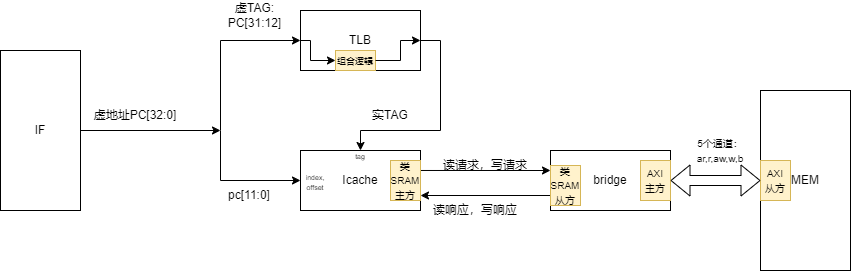
\includegraphics[width=\textwidth]{fig/fig3.png}
    \caption{ICache集成在CPU中示意图}
    \label{fig:3}
\end{figure}
\begin{enumerate}
    \item ICache与CPU的接口设计
    
由于Cache采用的是“虚Index实Tag”的方式,所以当cpu取指的时候,把虚拟地址的Index直接传递给Cache,Cache便开始根据虚拟地址的Index进行查询,

同时,将虚拟地址传递给虚实地址转换单元,它能通过组合逻辑在同一拍,将虚拟地址转换为物理地址的TAG,并传递给Cache。

上述方式使得Cache和TLB查询能并行执行,提高了效率。

    \item ICache与转接桥的接口设计
    
    Icache将访存请求发送到转接桥,转接桥将类sram的访存请求转换为AXI总线的访存请求,并且如果是多个字的访存请求,采用突发 burst 的方式。

    以写通道的burst控制为例,
    \begin{lstlisting}[language=verilog]
assign awlen =      awtype_reg == 3'b100 ? 8'd3 : 8'd0; // 如果是写整个cache行,burst长度为3
assign awsize =     3'b010; // 每拍发送一个字
assign awburst =    2'b01;  // 地址增加突发
assign wlast =      awtype_reg == 3'b100 ?wdata_cnt == 2'b11    // 最后一个字,拉高wlast
                    :1'b1;

always @(posedge clk)begin
    if(~resetn)begin
        wdata_cnt <= 2'b0;
    end
    else if(aw_current_state == AW_SEND_DATA && wready)begin
        wdata_cnt <= wdata_cnt + 1;
    end
end
    \end{lstlisting}

\end{enumerate}





\section{实验过程中遇到的问题、对问题的思考过程及解决方法(比如RTL代码中出现的逻辑bug,逻辑仿真和FPGA调试过程中的难点等)}

\noindent
$\bullet$
\textbf{TLB 搜索match出错}。


      
\vspace{1ex}

\section{小组成员分工合作情况}
王敬华负责TLB模块实现,部分TLB指令的添加和冲突的处理。

李霄宇负责TLB相关指令的添加,部分冲突的处理,接口连接。

艾华春负责添加TLB相关寄存器和TLB相关的例外支持,为cpu增加虚实映射功能。

实验报告为根据每人负责代码的部分,写相应部分的报告。
\end{document}